\chapter{Results} % Main chapter title

\label{results} % For referencing the chapter elsewhere, use \ref{Chapter1} 

\lhead{Chapter 4. \emph{Results}} % This is for the header on each page - perhaps a 

\section{Full System Tests}
\label{sec:fullsystest}

An initial test of the completed system was performed using parameters similar to those in figure \ref{fig:drvmatching}.  The complete conditions were as follows: 100000 8 dimensional points were generated following the same procedure in Section \ref{sec:inittest}.  The conditions for the ANN searches performed used a K of 20, and limited the number of nodes searched to 500.  This means that only about .5\% of the vector space was searched.  This test was performed using 80 different randomly generated DRVs, with 20 random points generated for each again following the procedure in Section \ref{sec:inittest}.  This means that each index was tested against 1600 different queries.  The same MPDG error metric is also used, which measures the ratio of the average distance between the points in each query's result set and that of a linear search.  For our system, the default parameters described in Section \ref{sec:myimpl} were used.

From figure FILL, it is clear that the SMS based k-d trees tend to perform significantly better than those with random weights.  Thus, even though the offline construction cost of the random method is lower (due to not requiring a linear seek across each dimension), it is worth investing in WSMS, as this is is a one time cost and leads to significant improvement in result quality.  In fact, a single k-d tree using SMS had higher overall performance than our system when using SPM.  It is also important to note that the query DRVs used were pulled from a uniform distribution using the same method described in section \ref{sec:inittest}.  As such, many of these DRVs were not drastically different from a standard uniform split.  Thus, while our data structure lead to a performance improvement for both splitting heuristics, the baselike k-d tree still performed rather well.

\begin{figure}[h]
\begin{center}
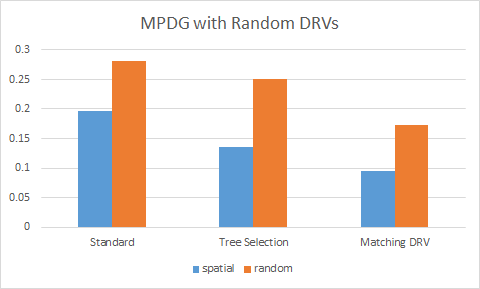
\includegraphics[width=.85\textwidth]{Figures/fullsysrand}
\end{center}
\caption{Full system test with random DRVs from uniform distribution}
\label{fig:fullsysrand}
\end{figure}

The real improvements came however from extreme queries which only use a small subset of dimensions.  The same parameters for our sytem were chosen with the exception of setting the DDD to 3, however the method of selecting the query DRVs was changed to only include a smaller subset of dimensions.  The method for doing so was to require a single dimension to be selected, and to determine whether or not other dimensions should be selected with a bernoulli random variable.  Thus, the distribution of the number of selected dimensions given a selection probability p and D dimensions is described by Binomial(D-1,p) + 1.  After selecting a subset of dimensions, the weight of each dimension was drawn randomly from a uniform distribution and normalized to a sum of one.  Of note is that when only one dimension is selected it will have a weight of 1 in the DRV, and it would be ideal to only split on that dimension.  Fortunitely, a seed DRV of all single dimension cases is included, and as such there is guaranteed to be a tree which perfectly matches, and only splits on that dimension.  In this case, the k-d tree performs equivalent to a binary search tree, and true nearest neighbors can be computed in O(Log(N)).  When more than one dimension is selected, while a perfect match tree likely won't exist (since weights are equal in seed DRVs), the two dimensional matching seed DRV will perform well if the query DRV is close to equal in the two dimensions, while the single dimension DRV will perform well when one dimension has a much larger weight than the other.

\begin{figure}[h]
\begin{center}
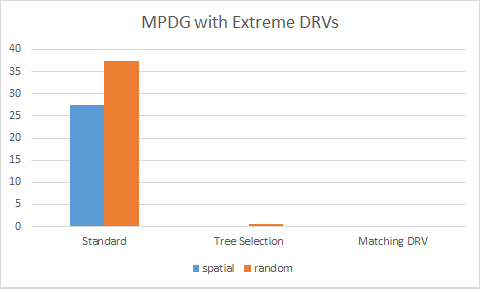
\includegraphics[width=.85\textwidth]{Figures/fullsysext}
\end{center}
\caption{Full system test with DRVs containing a low number of dimensions}
\label{fig:fullsysext}
\end{figure}

As shown in figure FILL, with extreme queries our data structure's performance was extremely close to the max possible performance with different DRVs, while the standard k-d tree performance decreased greatly.  Of course the true performance of our system likely lies somewhere in the middle of these cases shown in Figure FILL and FILL, as the true distribution of search queries likely lies somewhere in the middle.  Also of note is that seed DRVs with all sets of three dimensions were present, and nearly 85\% of the selected DRVs had three or less dimensions.  However, even when four to five dimensions are selected performance is still expected to be strong.

Because of the significantly higher performance of WSMS compared to SPM, future tests are performed only using the WSMS heuristic.  The key advantage to SPM is that all split dimensions are selected in constant time, wheras those in WSMS require a linear seek across all dimensions.  However, this cost is only associated with offline construction of the trees which is only performed once.  Since our benchmark attempts to optimize result quality on a live system, WSMS is a superior heuristic.  In \ref{sec:realworld}, we discuss that in a live system it may be necessary to reconstruct trees at times and as such, when performance tuning one should consider the merits of a heuristic with lower tree construction cost.

For future tests, unless otherwise specified, query DRVs were generated randomly with each dimension following the smae process used for the queries in Figure FILL.  Additionally, for future tests three different indexes were generated.  The first is a standard k-d tree for baseline performance.  The second is our system, using the standard parameters described above.  The final index generated is a singled k-d tree using WSMS with a seed DRV matching that of the query DRV.  This case represents hypothetical best case performance with our heuristics.

\section{Change of Dimensionality}

One important factor to test is how our system performs on data sets with different dimensionalities.  The dataset was again generated following the procedure from \ref{sec:inittest}; however, data was generated with different dimensions.

\begin{figure}[h]
\begin{center}
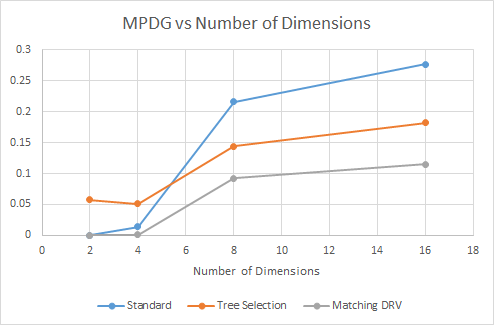
\includegraphics[width=.85\textwidth]{Figures/dims}
\end{center}
\caption{Full system test with data set of varying dimensions}
\label{fig:dim}
\end{figure}

The results for this test are shown in Figure FILL.  For each index, the MPDG increases with dimensionality.  This is to be expected, as performance for tree based indexes begins to degrade at higher dimensionalities.  Of note is that our system actually performed worse than a standard k-d tree for very low dimensionality.  This is likely because some searches were used to select the best trees.  Additionally, the k-d tree has the advantage of searching in a single tree, while searches in our index were split between multiple, and as seen in Figure FILL the performance of forests tends to be slightly worse than that of a single tree.  With a higher number of dimensions however, our system performs better than k-d trees, as the value of selecting trees with better seed DRVs is higher with more dimensions.

\section{Size of Dataset}

We also tested the performance of our system on datasets of varying size.  Again the same procedure from \ref{sec:inittest} was followed, but using a variety of different sizes.

\begin{figure}[h]
\begin{center}
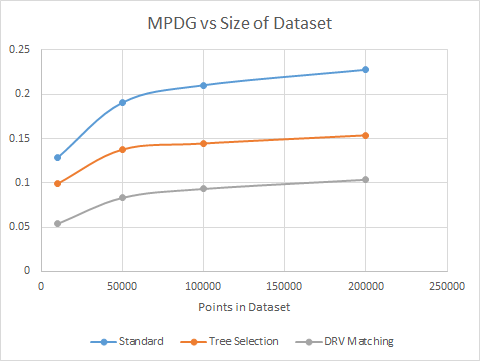
\includegraphics[width=.85\textwidth]{Figures/size}
\end{center}
\caption{Full system test with data set of varying size}
\label{fig:size}
\end{figure}

The results for this test are shown in Figure FILL.  For each of the indexes, the MPDG increases with the size of the dataset.  This is expected, as a larger dataset with a fixed number of nodes search means that a lower percentage of nodes are searched.  Of note is that the standard k-d tree index's performance decreased at a faster rate than that of our index and the tree with a matched seed DRV.  Thus, the benefits of our system are larger for bigger datasets. 

\section{Number of Trees}

The number of trees in our system is expected to have a direct impact on in its performance.  We tested our system against the same dataset described in \ref{sec:inittest}, generating our index with a varying number of random trees.

\begin{figure}[h]
\begin{center}
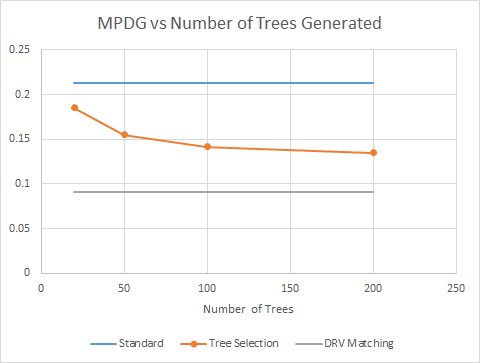
\includegraphics[width=.85\textwidth]{Figures/ntreesgen}
\end{center}
\caption{Full system test with varying number of random trees in our system}
\label{fig:ntreesgen}
\end{figure}

The results are shown in Figure FILL.  The orange line represents the performance of the standard k-d tree, while the grey line represents the performance of a tree with a matched seed DRV.  With a larger number of trees, the overall quality of of the selected trees will increase, since with more trees there are more chances for a high quality match.  However, this effect is diminishing.  As the number of trees increases, the performance increase from doing so drops.

\section{Nodes Searched}

\begin{figure}[h]
\begin{center}
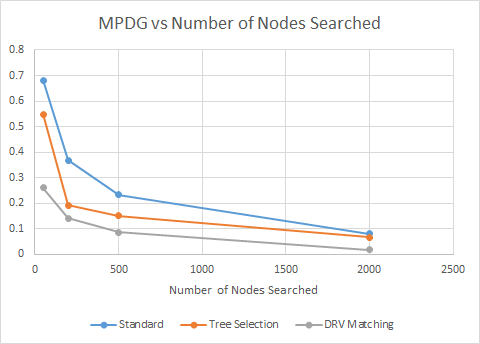
\includegraphics[width=.85\textwidth]{Figures/nsearch}
\end{center}
\caption{Full system test with varying number of nodes searched}
\label{fig:nsearch}
\end{figure}

We also considered the performance of our system for varying numbers of nodes searched.  The results for this test are shown in Figure FILL.  As expected, for each index, the MPDG decreases with an increase in the number of nodes searched.  This effect is dimishing however.  Initially, an increase in the number of nodes searched leads to a large decrease in MPDG, wheras a similar increase when a large number of nodes are already searched has little effect.  Also of importance is that for a very small number of nodes searched our system's performance is close to that of a standard k-d tree.  This is because a high proportion of the alloted searches are used to select which trees to search.  As the number of searches increases so does our system's performance relative to the standard k-d tree.  At a large enough number of searches, the standard k-d tree eventually catches up to our index.  Thus, our index was most effective when about .2\% to .5\% of the nodes were searched.

\section{Size of Result Set}

\begin{figure}[h]
\begin{center}
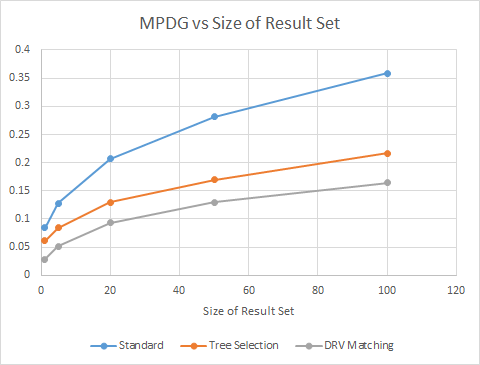
\includegraphics[width=.85\textwidth]{Figures/k}
\end{center}
\caption{Full system test with varying size of result set (K)}
\label{fig:kparam}
\end{figure}

\section{Number of Trees Per Query}

\begin{figure}[h]
\begin{center}
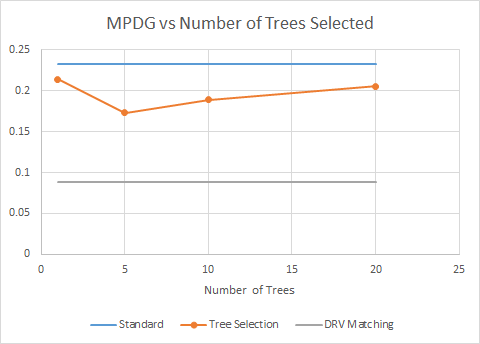
\includegraphics[width=.85\textwidth]{Figures/treesel}
\end{center}
\caption{Full system test with varying number of trees retrieved per query}
\label{fig:treesel}
\end{figure}

\section{Alternative Dataset}

http://archive.ics.uci.edu/ml/datasets/Corel+Image+Features
http://archive.ics.uci.edu/ml/machine-learning-databases/CorelFeatures-mld/CorelFeatures.data.html
\begin{figure}[h]
\begin{center}
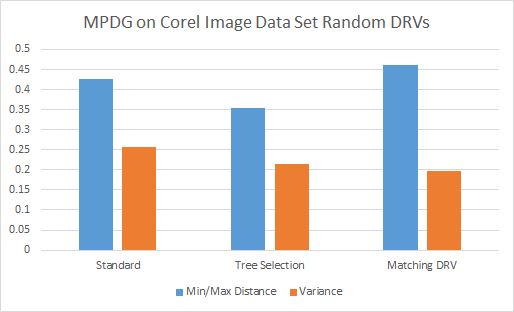
\includegraphics[width=.85\textwidth]{Figures/altrand}
\end{center}
\caption{Full system test on Corel Image Features Data Set with random DRVs from uniform distribution}
\label{fig:altrand}
\end{figure}

\begin{figure}[h]
\begin{center}
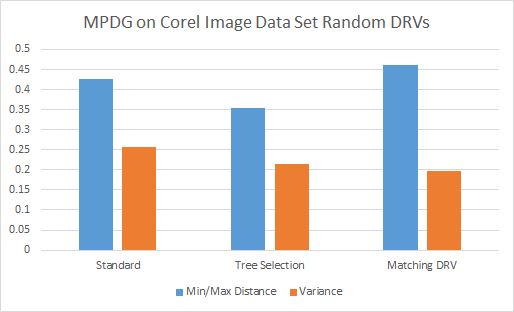
\includegraphics[width=.85\textwidth]{Figures/altext}
\end{center}
\caption{Full system test on Corel Image Features Data Set with DRVs with a low number of dimensions}
\label{fig:altext}
\end{figure}
check
